\subsection{Randomize Data}
\subsubsection{Time}
Execution time unit: milliseconds

\begin{table}[h!]
\centering
\begin{tabular}{|l|r|r|r|r|r|r|}
\hline
\textbf{Algorithm} & \textbf{10,000} & \textbf{30,000} & \textbf{50,000} & \textbf{100,000} & \textbf{300,000} & \textbf{500,000} \\ \hline
selection-sort & 90.9034 & 819.165 & 2144.86 & 8596.38 & 76158.2 & 210088 \\ \hline
insertion-sort & 5.4657 & 49.4609 & 138.977 & 547.006 & 4937.82 & 13827.8 \\ \hline
shell-sort & 20.9348 & 204.922 & 550.198 & 2260.1 & 18522.9 & 53320.1 \\ \hline
bubble-sort & 97.1671 & 1116.17 & 3208.09 & 13295.4 & 121053 & 339611 \\ \hline
heap-sort & 0.909 & 3.1648 & 5.3967 & 11.5898 & 39.6501 & 68.36 \\ \hline
merge-sort & 3.2503 & 9.3788 & 15.4051 & 28.9049 & 87.508 & 146.323 \\ \hline
quick-sort & 0.5708 & 1.7461 & 3.1067 & 6.3324 & 20.1092 & 34.9733 \\ \hline
radix-sort & 1.8813 & 0.5193 & 0.7778 & 1.8149 & 4.8387 & 8.4334 \\ \hline
counting-sort & 0.07 & 0.1945 & 0.2539 & 0.4312 & 0.902 & 1.3383 \\ \hline
binary-insertion-sort & 4.8785 & 37.591 & 102.974 & 410.325 & 3620.11 & 10357.5 \\ \hline
shaker-sort & 85.7846 & 842.283 & 2380.6 & 9535.75 & 86159.8 & 239150 \\ \hline
flash-sort & 0.1696 & 0.6379 & 0.9506 & 1.8552 & 7.8633 & 16.1854 \\ \hline
\end{tabular}
\label{table:running_time}
\end{table}

\begin{figure}[h]
    \centering
    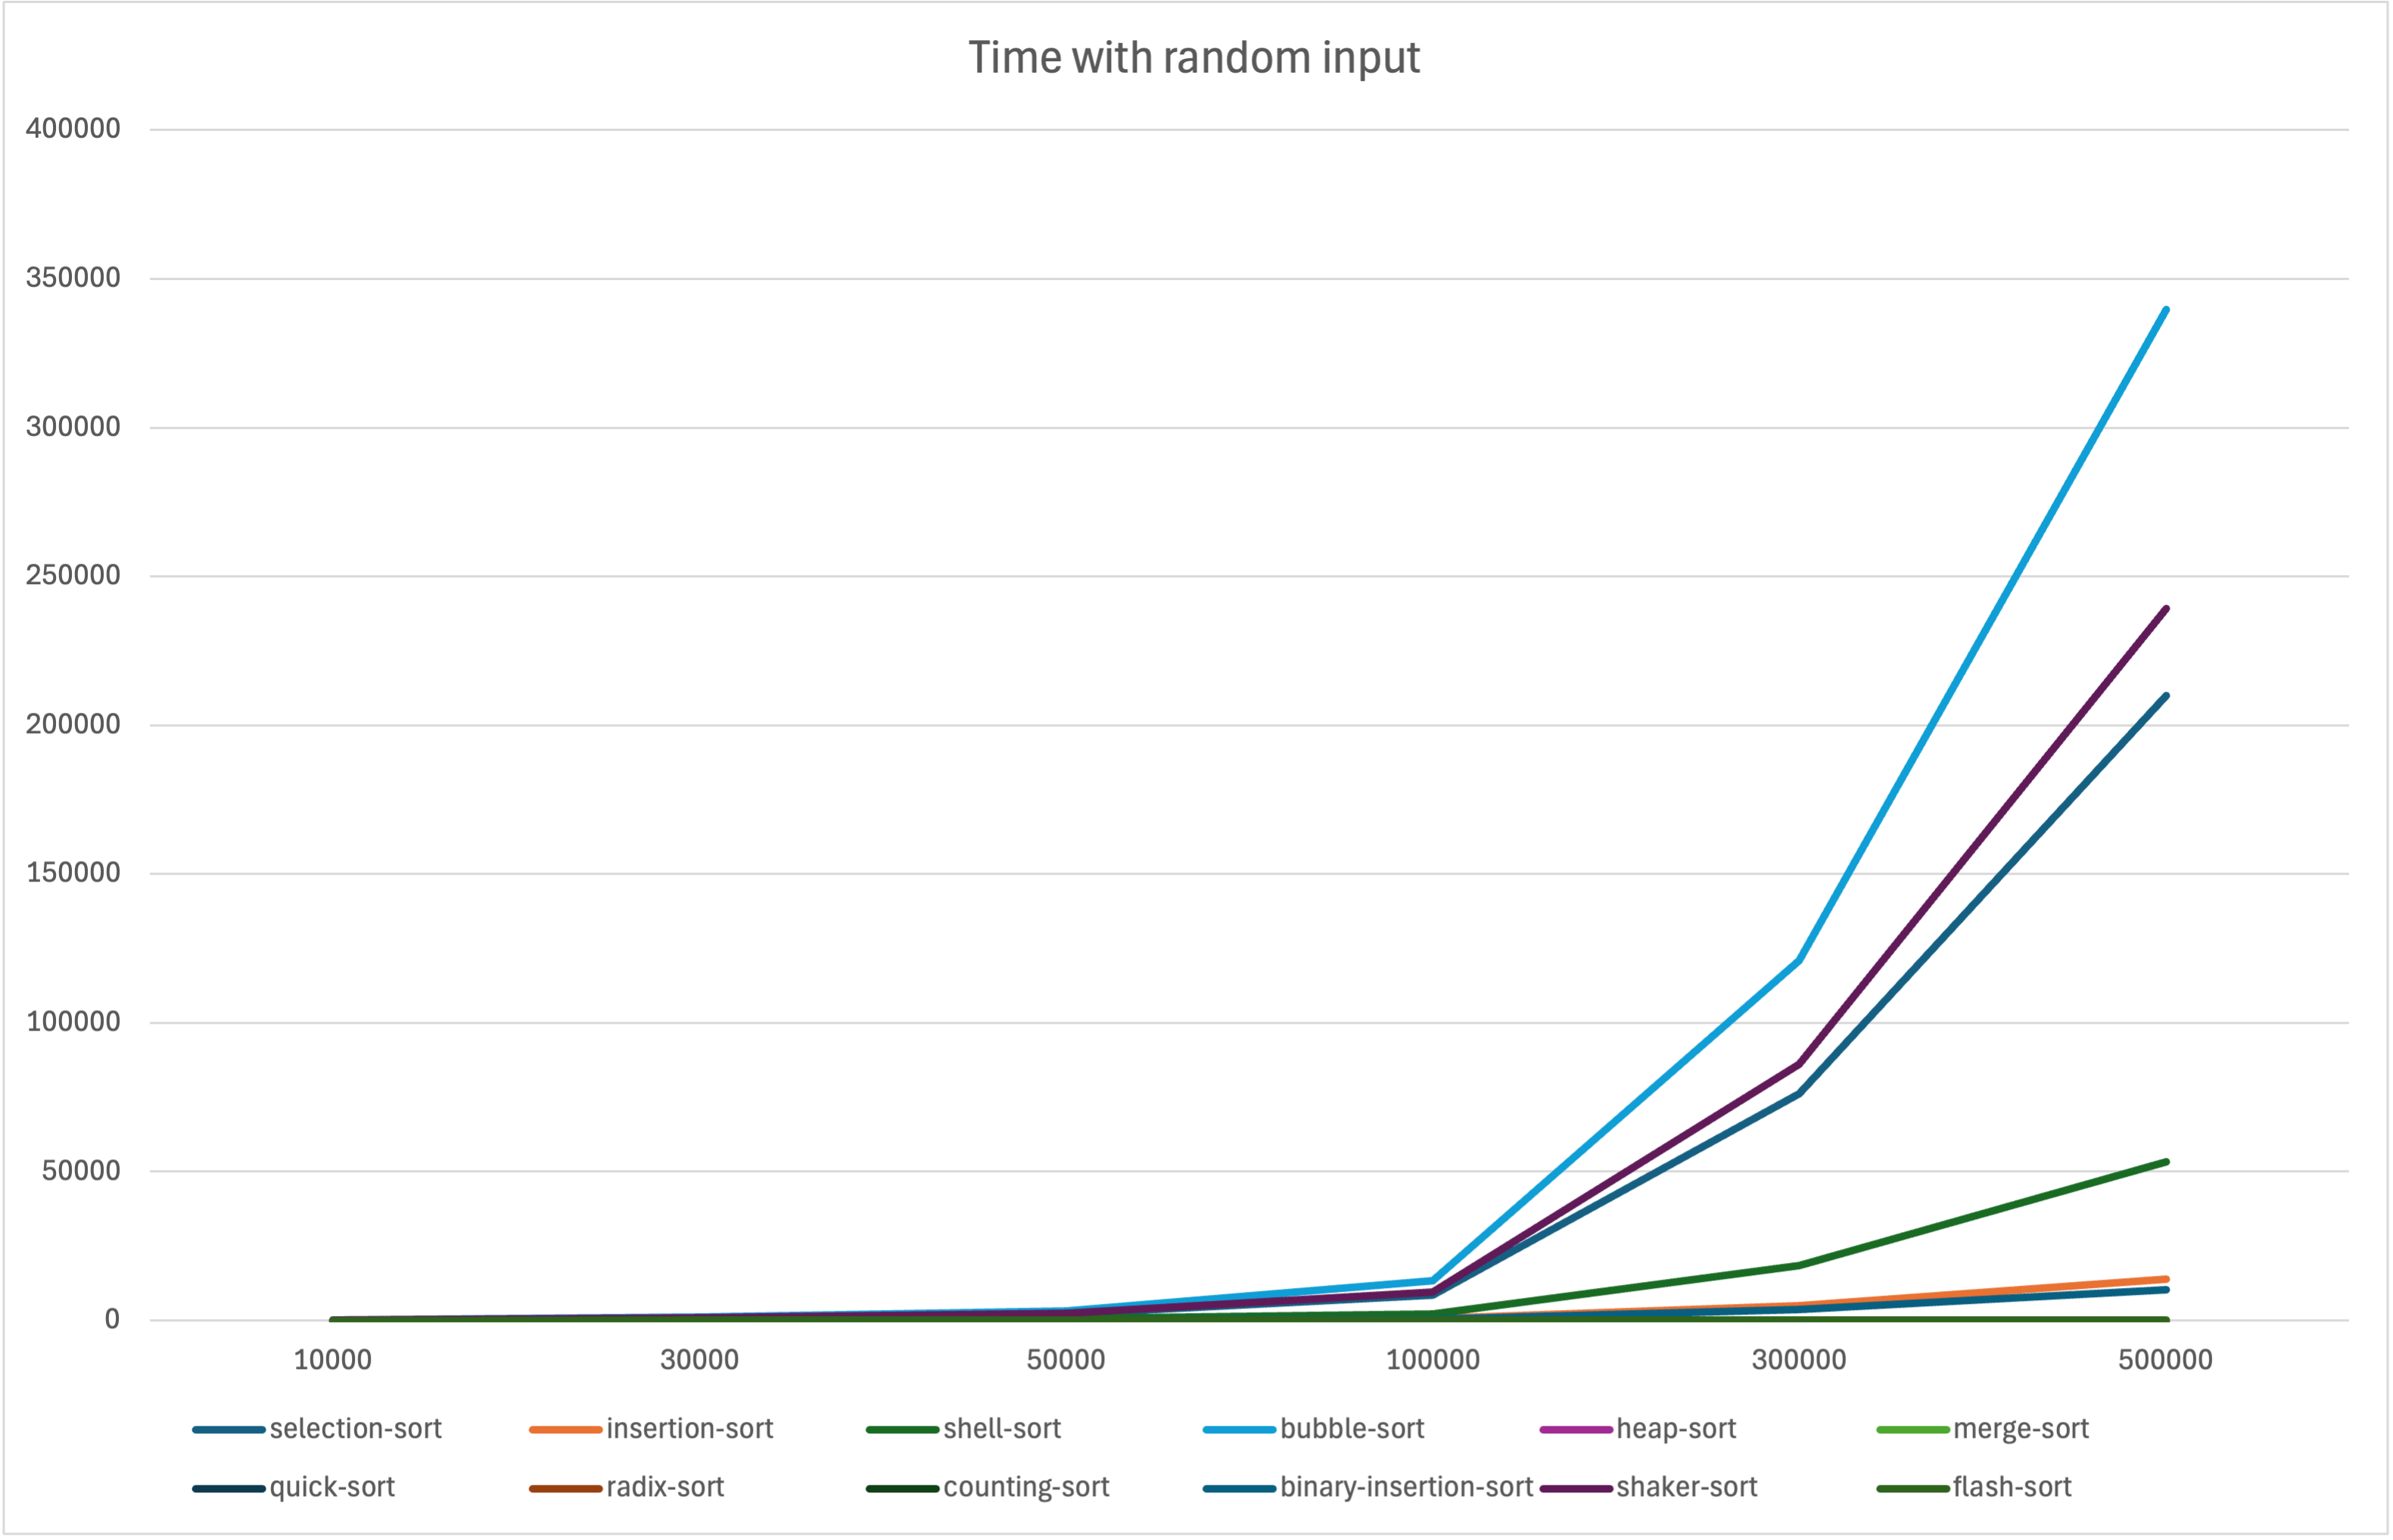
\includegraphics[scale=0.65]{Figures/Visualization/Random_time.png}
    \caption{Execution time for Randomize data}
    \label{fig:enter-label}
\end{figure}

\textbf{Comments on the running time of sorting algorithms with random data}
\begin{enumerate}
    \item \textbf{Fastest algorithms:} \\
   - \texttt{Counting Sort}, \textit{Quick Sort}, \textit{Heap Sort}, and \textit{Flash Sort} are the fastest algorithms as the data size increases. Notably, \textit{Quick Sort} and \textit{Flash Sort} have very low running times compared to other algorithms, even with large datasets like 500,000 elements.

    \item \textbf{Slowest algorithms:} \\
   - \textit{Bubble Sort}, \textit{Selection Sort}, and \textit{Insertion Sort} have the longest running times. \textit{Bubble Sort} and \textit{Selection Sort} have rapidly increasing running times, reaching hundreds of thousands of seconds with datasets of 500,000 elements.

    \item \textbf{Other algorithms:} \\
   - \textit{Merge Sort}, \textit{Shell Sort}, and \textit{Shaker Sort} have average running times, neither too fast nor too slow.
\end{enumerate}

\subsubsection{Comparison}
\begin{table}[h!]
\centering
\begin{tabular}{|l|r|r|r|r|r|r|}
\hline
\textbf{Algorithm} & \textbf{10,000} & \textbf{30,000} & \textbf{50,000} & \textbf{100,000} & \textbf{300,000} & \textbf{500,000} \\ \hline
selection-sort & 100020001 & 900060001 & 2500100001 & 10000200001 & 90000600001 & 250000000001 \\ \hline
insertion-sort & 49650481 & 448332712 & 1248140892 & 4990403035 & 45011022554 & 124964111984 \\ \hline
shell-sort & 136486703 & 1228074234 & 3411144570 & 13643867417 & 1.2279e+11 & 3.41082e+11 \\ \hline
bubble-sort & 100009999 & 900029999 & 2500049999 & 10000099999 & 90000299999 & 2.5e+11 \\ \hline
heap-sort & 638069 & 2149637 & 3772566 & 8044375 & 26494137 & 45968203 \\ \hline
merge-sort & 583723 & 1937626 & 3383060 & 7166134 & 23383144 & 40382087 \\ \hline
quick-sort & 364891 & 1086464 & 1921044 & 4144209 & 14922110 & 27756867 \\ \hline
radix-sort & 140051 & 510064 & 850064 & 1700064 & 510064 & 850064 \\ \hline
counting-sort & 60001 & 180001 & 265539 & 465539 & 1265539 & 2065539 \\ \hline
binary-insertion-sort & 25432305 & 226953151 & 629328887 & 2511144485 & 22498338748 & 62537270911 \\ \hline
shaker-sort & 66785983 & 599351162 & 1667586501 & 6658782743 & 60022078477 & 1.66739e+11 \\ \hline
flash-sort & 92801 & 285860 & 496012 & 892630 & 2755320 & 4583014 \\ \hline
\end{tabular}
\label{table:comparisons}
\end{table}

\begin{figure}[h]
    \centering
    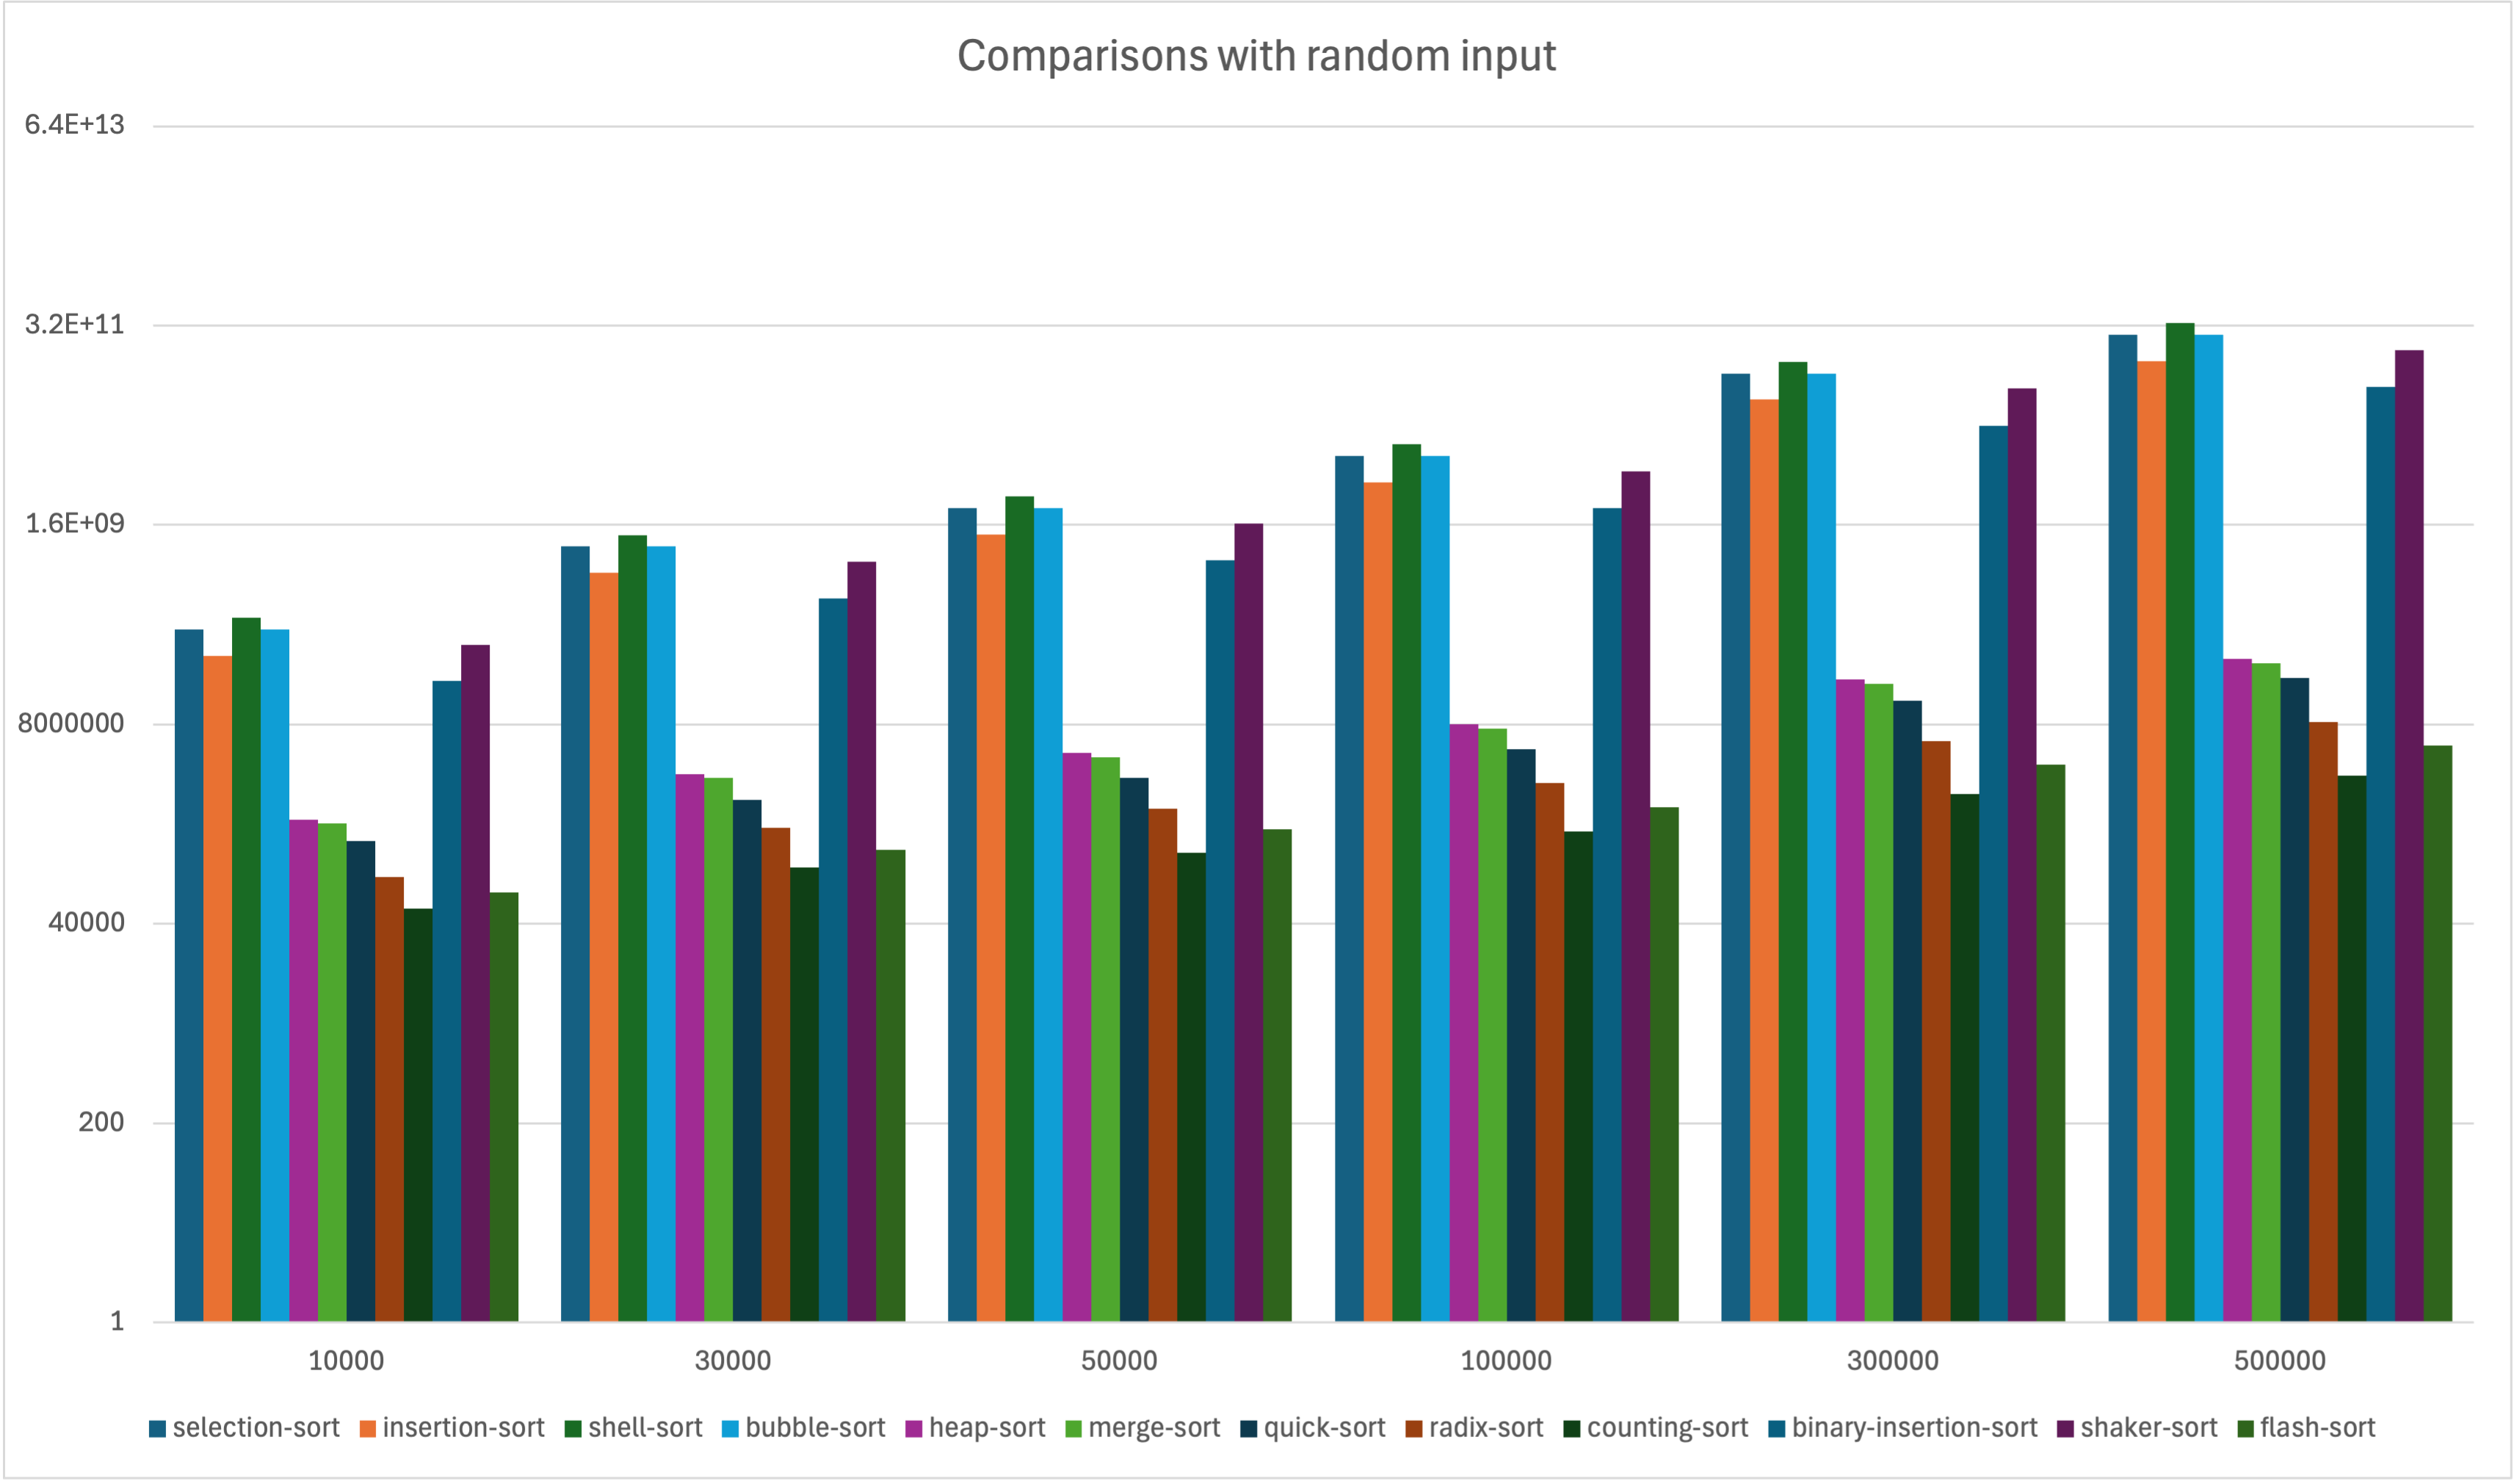
\includegraphics[scale=0.65]{Figures/Visualization/Random_compare.png}
    \caption{Number of comparisons of the algorithm for Randomize data}
    \label{fig:enter-label}
\end{figure}

\textbf{Comments on the number of comparisons of sorting algorithms with random data}
\begin{enumerate}
    \item \textbf{Fewest comparisons:} \\
   - \textit{Counting Sort}, \textit{Flash Sort}, and \textit{Radix Sort} have the fewest comparisons, especially \textit{Counting Sort}, which has very low comparison counts even with large datasets.

    \item \textbf{Most comparisons:} \\
   - \textit{Bubble Sort}, \textit{Selection Sort}, and \textit{Insertion Sort} have very high comparison counts, especially \textit{Bubble Sort} and \textit{Selection Sort}, which reach billions of comparisons with datasets of 500,000 elements.

    \item \textbf{Other algorithms:} \\
   - \textit{Quick Sort}, \textit{Heap Sort}, and \textit{Merge Sort} have relatively low comparison counts, making them more efficient compared to slower sorting algorithms.
\end{enumerate}

\subsubsection{Overall}
\textbf{Overall comments on algorithms based on all data and size}

\begin{enumerate}
    \item \textbf{Overall fastest algorithms:} \\
   - \textit{Quick Sort}, \textit{Heap Sort}, and \textit{Flash Sort} are the overall fastest algorithms. Among them, \textit{Quick Sort} is most commonly used due to its efficiency in handling large datasets.

    \item \textbf{Overall slowest algorithms:} \\
   - \textit{Bubble Sort}, \textit{Selection Sort}, and \textit{Insertion Sort} are the overall slowest algorithms. They are suitable only for very small datasets or educational purposes.

    \item \textbf{Stable and unstable algorithms:} \\
   - Algorithms like \textit{Merge Sort} and \textit{Insertion Sort} are stable, meaning they maintain the relative order of equal elements. \\
   - Algorithms like \textit{Quick Sort} and \textit{Heap Sort} are unstable, meaning they do not maintain the relative order of equal elements.
\end{enumerate}
